\documentclass{article} % For LaTeX2e
\usepackage{nips, times}
\usepackage{hyperref}
\usepackage{url}
\usepackage{graphicx}
\usepackage{amsmath}
\usepackage{amssymb}
\usepackage{booktabs}
\usepackage{tabularx}
\usepackage{caption}
\usepackage{subcaption}
\usepackage{color}
\usepackage{relsize}
\usepackage{placeins}
\usepackage{natbib}
\usepackage{paralist}
\usepackage{bbm}
\usepackage{subfigure}
\usepackage{multirow}
\usepackage{enumitem}
\usepackage[toc,page]{appendix}

\renewcommand{\null}{\operatorname{null}}
\newcommand{\given}{\,|\,}

\input math.tex

\nipsfinalcopy

\begin{document}
\title{Image Segmentation using superpixel based MRF and shape priors}

\author{
Fanny Yang\\
University of California\\
Berkeley, CA 94720, USA\\
\texttt{fanny-yang@eecs.berkeley.edu} \\
\And
Siqi Wu\\
University of California\\
Berkeley, CA 94720, USA\\
\texttt{siqi@stat.berkeley.edu}\\
}

\maketitle

\section{Introduction}
Gene expression analysis relies on photographic material of fruitfly embryos. However for each embryo, a different embryo had to be used. Especially in later stages of the development the organs like mouth, gut and the yolk all lie in slightly different locations and have different shapes. In order to achieve comparability of the gene expressions in these different variations one needs to map the embryos to a standard template. One measure to achieve this is to segment the different organs and derive a map thereof. 

In the problem that we tried to tackle, the embryos are already considered to be in the same position and right rotation. The code had already been written to achieve that. Therefore one is left with the image segmentation task within the embryo, where the organs are very hard to discern even for the human eye. This is for example due to almost very little intensity variation and almost no color information.

In the following I will quickly outline a few commonly used image segmentation algorithms which are relevant for this paper and some difficulties when applying them to the current problem. This will then lead to the motivation for the proposed algorithm which combines some of the ideas to form a new segmentation algorithm.

\section{Previous works}
All of the models have in common that they the segmentation task is equivalent to the minimization of some energy cost function, with each of them having an equivalent interpretation in terms of maximizing a posterior distribution. 

\paragraph{Deformable models}
For example, one line of method, categorized in this paper as deformable models is based on the idea of Snakes \cite{Kass88_Snakes, Cootes92_ActiveShape,Cootes01_ActiveApp, Cootes92_TrainingShape}, also called ``Active Contours''. The decision variable they optimize over is a parameterized contour $c(s)$, by a point distribution model. In the very early and simple model, the energy consists of the length and smoothness of the curve which is the internal energy (image independent), and a term called the external energy which measures how much it is consistent with the edge image, i.e.
\beqs
E(\tilde{I},c) = E_{ext}(c) + E_{int}(I,c) = \int_0^1 \tilde{I}(c(s))\d s  + \int_{\Omega} \alpha(s)|c'(s)|^2 + \beta(s)|c''(s)|^2\d s
\eeqs
where $\tilde{I}$ here is the edge image.

\cite{Sclaroff01_RegionGroup, ElBaz09_ShapeApp}
% Level set 
Since the parameterization of the curve is usually cumbersome, people have proposed modelling the contour $c$ as the zero level set of a continuous function $\phi(x,y)$ \cite{Caselles97_Geodesic, Leventon00_ShapeGeodesic, ChanVese01, MumfordShah89,Cremers07_Levelreview, Tsai03_MILevelSets}. The energy minimization decision variable is then a function which thus requires techniques from functional analysis, in particular partial differential equations (PDE) e.g. using Euler-Lagrange equations. Later this framework was extended to enable incorporation of shape and intensity priors \cite{Cremers06_KernelDensity, Chan05_LevelShape, Chen09_LevelShapeIntensity}.

The advantages of level set segmentation methods are that, if correctly used, can be used to find global optima 
%Good:
%Bad: 

\paragraph{Graphical models}
Another line of work has concentrated on the probabilistic interpretation of energy minimization which is maximum likelihood estimation. The labels $y$ are treated as unknown variables while the image features $x$ (e.g intensity, texture etc.) are treated as observables (more details in section ???). There are mainly two different approaches: The discriminative approach (conditional random fields \cite{Lafferty01_CRFSeq, KaeSohn13_CRF}) models $p(y|x)$ directly, where as the generative approach (Markov random fields) models $p(x|y)$ as a Gaussian distribution and uses pairwise potentials $p(y_i,y_j)$ for neighboring pixels and potentially priors on the label. CRF methods generally need more training data whereas MRF are fairly self-sufficient.

These maximum likelihood problems are generally impossible to solve exactly since the graphical model is not a tree so that one has to use loopy belief propagation or variational inference methods (???). However for binary segmentation the GraphCut algorithm for example (???) is able to solve the problem precisely under the condition that the cost function is a submodular quadratic pseudo-boolean function of the form
\beqs
E(y) = a + \sum_i a_i y_i + \sum_{i,j}a_{ij}y_i y_j
\eeqs
where $y_i\in {0,1}$ for each $i$ and possibly depend on the observations $x$. 

A common problem for these approaches is that they often find local structures but cannot incorporate global information. Several unsupervised and supervised extensions have thus been brought forth such as using Restricted Boltzmann machines \cite{KaeSohn13_CRF}, multiscale representations of the feature space \cite{He04_MultiScale} and shape priors \cite{Lempitsky_BranchMin}.


\paragraph{Hybrid models and superpixels}
There have already been attempts to combine the two frameworks \cite{Huang04_MRFDM, Chen12_MIGraphCut, Uzunbas13_MultiOrgan, Schlesinger13}. 
However pixelwise MRF/CRF are computationally inefficient to solve for high resolution images as is the case in our segmentation task. In this case we exploit the work by Malik et al. \cite{Malik_Superpixel} and pre-process the high-resolution images using their superpixel algorithm. This clusters regions according to their texture and brightness similarity as well as contour cues using trained data from natural images (???).
%In order to find the organs automatically we need to have a reasonably high number of superpixels such that the real contour is actually in the set of possible edges given by the superpixel edges. It should also not be too high since edges tend to become very non-smooth. 

The first attempts which were made to segment e.g. the gut used superpixels at different scales and applied a random forest algorithm on these superpixels. Similarly a CRF and Restricted Boltzmann machines were tested on the data. However, albeit being accurate for some of the images, it could not provide a very reliable segmentation result throughout the range of different embryos. 

Since for each life stage of the embryo, it is known to have a structure similar to a given template, we want to incorporate this prior information into an superpixel based MRF approach.  
The level set segmentation framework provides an easy way to incorporate such priors, where the probability distribution over the shapes is calculated using Gaussian kernel density estimation.

\section{Model}

In our novel model we use an MRF similar to the one in \cite{Huang04_MRFDM}, however we do not use contours which carry the burden of parameterization but take advantage of the level set functions. Also later on we extend this framework to the super pixel level.

We first describe the model on a pixel level. Let's denote $y$ as our hidden labels, $x$ as our observed image intensities (in principle this can be any feature). We index pixels by $i$ and our signed distance function is $\phi$. For our joint probability distribution we use a undirected graphical model as in figure ??? with node set $\Nu$ and edge set $E$. 
This yields the following factorization using pairwise and singleton potentials 
%Our graphical model, depicted in ??? allows for the following factorization with pairwise potentials $\psi$ reads
\begin{align}
p(x,y,\phi) &=  \prod_{i\in \Nu} \psi(x_i,y_i)  \prod_{(i,j)\in E} \psi(y_i,y_j)\prod_{i\in \Nu} p(y_i|\phi)p(\phi) \label{total_joint}\\
&=: \prod_{i\in \Nu} p(x_i|y_i)p(y_i,y_j)p(y_i|\phi)p(\phi|\tilde{\phi})\nonumber
\end{align}
where $\tilde{\phi}$ denote prior shapes.
In general the edge structure does not necessarily have to be a lattice.

We model $p(x_i|y_i)$ as Gaussians with parameters $\mu_{y_i}$ and $\sigma_{y_i}$, i.e. 
\beqs
p(x_i|y_i) = \frac{1}{\sqrt{2\pi}\sigma_{y_i}}\exp(-\frac{(x_i-\mu_{y_i})^2}{2\sigma_{y_i}^2})
\eeqs

Our pairwise potentials read
\beqs
p(y_i,y_j) \propto \theta_1 \Indi_{y_i\neq y_j} + \theta_2 \Indi_{y_i=y_j}
\eeqs
%It turns out that the choice of $\theta_i$ is best made using the observed $x_i, x_j$. 

For the consistency measure of the labels $y$ on $\phi$ we use the logistic function
\beqs
p(y_i|\phi) = \left(\frac{1}{1 + \E^{-\lambda \phi(i)}}\right)^{y_i} \left(\frac{1}{1 + \E^{\lambda \phi(i)}}\right)^{1-y_i}
\eeqs
where $\phi(i)$ is basically a signed distance function (possibly other distances) and $\lambda$ controls the sharpness of the slope. 
%Note: Schlesinger uses $\psi(y|\phi) = \E^{\sum_i y_i \phi(i)}$.

For the probability distribution on the level set function we use
\begin{align*}
p(\phi|\tilde{\phi}) &= E_{int}(\phi) + E_{prior}(\phi)\\
&= \lambda_1 \int_{\Omega}\delta_\epsilon(\phi(x,y))\|\nabla \phi(x,y)\|\d x \d y + \lambda_2 \int_{\Omega}H_\epsilon(\phi(x,y))\d x \d y\\
&- \log \sum_{i=1}^N \exp\left(-\frac{1}{2\sigma^2}d^2(H(\phi),H(\phi_i))\right)
\end{align*}
where $d$ is the smoothed symmetric distance between the level set functions defined as
\beqs
d^2(H_\epsilon(\phi_1),H_\epsilon(\phi_2)) = \int_{\Omega} (H_\epsilon(\phi_1) - H_\epsilon(\phi_2))^2 \d x\d y
\eeqs
Instead of using the non-smooth Heaviside function we apply a smoothed version, i.e. 
\beqs
H_\epsilon(z) = \frac{1}{2}(1+ \frac{2}{\pi}\arctan \left( \frac{z}{\epsilon} \right))
\eeqs
as in \cite{ChanVese01} with derivative $\delta_\epsilon(z) = \frac{\epsilon}{z^2 + \epsilon^2}$. The $\epsilon$ is dropped in the following for simpler notation.

\subsection{Structured Variational inference}
The inference task is to maximize $p(y,\phi|x) \propto p(x,y,\phi)$. However finding the maximum of \eqref{total_joint} exactly is computationally intractable. Therefore we use structural variational inference \cite{Jordan99_Variational, Wainwright_Variational} to approximate the problem, in which we look for a distribution $Q(y,\phi|x,a,b)$ which has a structure parameterized by $a,b$ that simplifies maximum likelihood computation. The ``best-matching'' $Q$ is found by minimizing the Kullback Leibler divergence $KL(Q||P) = \sum_\phi \sum_y Q(y,\phi|x,a,b) \log \frac{Q(y,\phi|x,a,b)}{p(y,\phi|x)}$. 

Our ansatz for the structure of $Q$ is the following factorization.
\beqs
Q(y,\phi|x,a,b) = Q_M(y|x,a)Q_D(\phi|b) 
\eeqs
with $Q_M(y|x,a) = \prod_{i,j} \psi(y_i,y_j) \prod_i  \xi(x_i,y_i) p(y_i|a_i)$ and $Q_D(\phi|b) \propto \prod_i p(b_i|\phi) p(\phi)$ so that we have factorized the distribution with respect to the two unknown vectors $y, \phi$. We are hence assuming independence of the two, given $a,b$ respectively.

We now need to minimize the KL divergence for which we follow the easy derivation in Blei:
Using the independence we can write out the KL 
\begin{align*}
&\EE \log Q_M(y|x,a) + \EE \log Q_D(\phi|b) - \EE \log p(y,\phi|x)\\
 = &\EE \left[\log Q_M(y|x,a)|\phi \right] + \EE \left[ \log Q_D(\phi|b) |y\right] - \EE \left[\EE \log p(y|\phi) |\phi \right]- \EE \log p(\phi)\\
= &\EE_{Q_M} (\log Q_M(y|x,a) - \EE_{Q_D} \log p(y|\phi)) + \EE_{Q_D} (\log Q_D(\phi|b) - \log p(\phi))\\
= &\EE_{Q_M} (\log Q_M(y|x,a) - \EE_{Q_D} \log p(y|\phi)) + \EE_{Q_D} (\log p(b|\phi) + c)
\end{align*}
where the first equality follows from the conditional independence of $y,\phi$ given $a,b$ and the second uses $Q_D(\phi) = p(\phi)$.

By Lagrange equations of first kind to incorporate the constraint of $\EE Q_D(\phi|b) |b = 1$ and $\EE Q_M(y|x,a) |x,a = 1$  we obtain that the Lagrange multiplier $\lambda = 1$ and the following mu
st hold for optimal $a,b$:
\begin{align*}
& -\EE_{Q_D} \log p(y|\phi) + \log Q_M(y|x,a) = 0\\
\implies  &\sum_i (\EE_{Q_D}\log p(y_i|\phi) - \log p(y_i|a_i)) = \sum_{j\in N(i)} \log p(y_i,y_j) - \EE_{Q_D} \log(p(y_i,y_j)) \\
\implies &\log p(y_i|a_i) = \EE_{Q_D} \log p(y_i|\phi) 
\end{align*}
and similarly
\begin{align*}
&- \EE_{Q_M} \log p(y|\phi) + \log p(b|\phi) = 0\\
\implies &\log p(b_i|\phi) = \EE_{Q^i_M} \log p(y_i|\phi)  
\end{align*}
where $Q_M^i = Q_M(y_i|x,a)$.

These are the fixed point equations and we will aim at solving them iteratively using alternating minimization. 

\subsection{Algorithm}

We now turn to the algorithm pipeline
. 
\paragraph{Algorithm}
Initialize level set function $\phi$.
Step $k$.
\begin{enumerate}
\item HOW DO WE do this first step - we only cover a region of $\phi$ for the steps?
\item Calculate $\phi^* = \argmax_{\phi} Q_D(\phi|b)$ using the current $p(b|\phi)$ and approximate by $Q'_D(c|b) = \delta(\phi^*)$
\item Calculate $p(y_i|a_i) = \exp(\EE_{Q'_D} \log p(y_i|a_i))= p(y_i|\phi^*)$.
\item In order to calculate $Q_M(y_i|x_i,a)$ estimate the parameters of $p(x_i|\theta_i)$ which are $\mu_1,\mu_0,\sigma_1,\sigma_0$ using the latent variable $y_i$ and the EM algorithm
\item Calculate $\log p(b_i|\phi) = \EE_{Q_M^i} \log p(y_i|\phi)$.
\end{enumerate} 

\subsection{Step 4 - EM algorithm using loopy belief propagation}
We now turn to the step of estimating the parameters of the Gaussians $p(x_i|y_i)$ for $Q_M(y|x,a)$ for which we will use an EM algorithm. The aim is to calculate 
\beqs
\max_{\theta} p(x|\theta,a) = \sum_y p(x,y|\theta) = \sum_y p(x|y,\theta)p(y|a)
\eeqs
For the EM algorithm we have the E Step
\begin{align*}
\L(q^{(t+1)},\theta) &= \sum_y p(y|x,\theta^{(t)}) (\log p(x|y,\theta) + \log p(y|a)) \\
&= \sum_i \sum_{y_i} \log p(x_i|y_i,\theta) \sum_{y_j:j\neq i} p(y|x,\theta^{(t)},a) + c(\theta)\\
%&= \sum_i \sum_{y_i} p(y_i|x, \theta^{(t)},a) \log p(x_i|y_i,\theta) + c(\theta)\\
&= \sum_i \sum_{y_i} p(y_i|x, \theta^{(t)},a) \Indi_{y_i=l} (-\log \sigma_l - \frac{(x_i -\mu_l)^2}{2\sigma_l^2}) + c(\theta)\\
&= \sum_i \sum_l p(y_i = l|x,\theta^{(t)},a) (-\log \sigma_l -  \frac{(x_i -\mu_l)^2}{2\sigma_l^2}) + c(\theta)
\end{align*}

For the maximization step we maximize $\L(q^{(t+1)},\theta)$ over $\theta$ so that we have
\begin{align*}
\mu_l^{(t+1)} &= \frac{\sum_i p(y_i=l|x,\theta^{(t)},a) x_i}{\sum_i p(y_i=l|x,\theta^{(t)})}\\
\sigma_l^{2(t+1)} &= \frac{\sum_i p(y_i =l | x,\theta^{(t)},a)(x_i-\mu_l)^2}{\sum_i p(y_i = l|x,\theta^{(t)},a)}
\end{align*}
which intuitively just computes the average intensity/variance within one label.

As we see we need to compute the marginal likelihood 
\beqs
p(y_i|x,\theta^{(t)},a) \propto \sum_{y_j:j\neq i} \prod_i p(x_i|y_i) \prod_{i,j} p(y_i,y_j) \prod_i p(y_i|a_i)
\eeqs
This can be readily computed using a loopy belief propagation algorithm/junction tree algorithm (slow?).
%% We write down the complete likelihood
%% \beqs
%% p(x_i|\theta_i) = p(y_i=1|a_i)p(x_i|y_i=1,\theta_1) + p(y_i=0|a_i)p(x_i|y_i=0,\theta_0)
%% \eeqs
%% We need to maximize this likelihood. 


\subsection{Step 2- Finding the level set function}
\label{levelset}
\subsubsection{Level Set Segmentation with prior}
The term $p(\phi)$ enables us to incorporate priors and regularizations. In our model we use length and area as in \cite{Cremers06_KernelDensity, ChanVese01, MumfordShah89}. Note that instead of $p(x|\phi)$ in level set formulations we now have $p(x|y)$ and $p(y|\phi)$.
\begin{align*}
-\log p(\phi|\tilde{\phi}) &= E_{int}(\phi) + E_{prior}(\phi)\\
&= \lambda_1 \int_{\Omega}\delta_\epsilon(\phi(x,y))\|\nabla \phi(x,y)\|\d x \d y + \lambda_2 \int_{\Omega}H_\epsilon(\phi(x,y))\d x \d y\\
&- \log \sum_{i=1}^N \exp\left(-\frac{1}{2\sigma^2}d^2(H(\phi),H(\phi_i))\right)
\end{align*}
where $H$ is the Heaviside function and $\sigma^2$ is the width of the Gaussian kernel. $E_{int}$ denotes the regularization on length and area of the region (boundary), $E_{prior}$ is the energy given by the shape prior which is measured as a distance $d^2(H(\phi),H(\phi_i)) = \int_{\Omega}(H(\phi)-H(\phi_i))^2\d x$ is basically doing a nonparametric kernel density estimation for the shape distribution using given samples $\phi_i$. We choose for the kernel width $\sigma^2=\frac{1}{N}\sum_{i=1}^N \min_{j\neq i}d^2(H(\phi_i),H(\phi_j))$.


The task is now to maximize $\log Q_D(\phi|b) \propto \log p(b_i|\phi)p(\phi)$ which is equivalent to minimizing the energies $E_{int}, E_{prior}$. By the multivariate Euler Lagrange equations (cite L.C. Evans) we know that $F(x) = \int \L(x,\phi(x),\nabla \phi(x))\d x$ is minimized if 
% for which Euler-Lagrange equation for multivariates $x$ yields the following fixed point equation for the optimal $\phi^*$:
\beqs
\frac{\partial}{\partial \phi} \L(x,\phi(x),\nabla \phi(x))  + \divop \frac{\partial}{\partial \nabla \phi} \L(x,\phi(x),\nabla \phi(x))=0
\eeqs 

We now add time for the evolution of the function and minimize the energy with respect to $\phi$ using the update equation
\begin{align}
\frac{\partial \phi}{\partial t} &= -\frac{\partial E_{int}(\phi)}{\partial \phi} - \frac{\partial E_{prior}(\phi)}{\partial \phi}  \label{labelset_update}\\
&=  \delta_{\epsilon}(\phi) (\lambda_1 \left[\divop(\frac{\nabla \phi}{\|\nabla \phi\|})\right] +\lambda_2) - \frac{\sum_i \alpha_i \frac{\partial}{\partial \phi} d^2(H(\phi),H(\phi_i))}{2\sigma^2 \sum_i \alpha_i}\nonumber
\end{align}
with $\alpha_i = \exp(-\frac{d^2(H\phi,H\phi_i)}{2\sigma^2})$.
This is basically doing a gradient descent. For the second term since $E_{prior}$ is a direct function of $\phi$, we can readily take the partial derivative with respect to $\phi$. $\frac{\partial}{\partial \phi} d^2(H(\phi),H(\phi_i))}
$ is a Gateaux derivative and yields
\beqs
\frac{\partial}{\partial \phi} d^2(H(\phi),H(\phi_i)) = \delta_{\epsilon}(\phi)(H(\phi)-H(\phi_i))
\eeqs

The question is how we can discretize the continuous first term in \eqref{labelset_update}. If we expand it we obtain
\beqs
\divop \frac{\nabla \phi}{\|\nabla \phi\|} = \frac{ \frac{\partial^2 \phi}{\partial x^2} (\frac{\partial \phi}{\partial y})^2 - 2 \frac{\partial^2 \phi}{\partial x \partial y} \frac{\partial \phi}{\partial x}\frac{\partial \phi}{\partial y} +  \frac{\partial^2 \phi}{\partial y^2} (\frac{\partial \phi}{\partial x})^2}{(\frac{\partial \phi}{\partial x}^2  + \frac{\partial \phi}{\partial y}^2)^{\frac{3}{2}}}
\eeqs
In our implementation we simply approximate the continuous derivatives by finite differences (this is exactly the formula they use in the Chan Vese Matlab package).

The overall formula for the update thus reads
\begin{align*}
\frac{\partial \phi}{\partial t} &= \delta_{\epsilon}(\phi)(\lambda_1  \frac{ \frac{\partial^2 \phi}{\partial x^2} (\frac{\partial \phi}{\partial y})^2 - 2 \frac{\partial^2 \phi}{\partial x \partial y} \frac{\partial \phi}{\partial x}\frac{\partial \phi}{\partial y} +  \frac{\partial^2 \phi}{\partial y^2} (\frac{\partial \phi}{\partial x})^2}{(\frac{\partial \phi}{\partial x}^2  + \frac{\partial \
phi}{\partial y}^2)^{\frac{3}{2}}} + \lambda_2) \\
&- \frac{\sum_i \alpha_i  \delta_{\epsilon}(\phi)(H(\phi)-H(\phi_i))}{2\sigma^2 \sum_i \alpha_i}\nonumber
\end{align*}


\paragraph{Notes}
The hard things are the length and also the derivative of the Heaviside function, which is a $\delta$ distribution. Instead of getting a very sharp boundary we introduce a mollified continuous Heaviside $H_{\epsilon} = $.

\subsubsection{Combining MRF with Level Set}
The coupling of the two frameworks happens in the step when we calculate the minimum of
\beqs
-\log Q_D(\phi|b) = -\log p(b|\phi) - \log p(\phi) = - \log p(\phi) - \EE_{Q_M^i}\log p(y_i|\phi)
\eeqs
We can use our results derived in section \ref{levelset} and arrive at the update step
\begin{align*}
\frac{\partial \phi}{\partial t} &= \frac{\partial}{\partial \phi} \log p(\phi) -\EE_{Q_M^i} \frac{\partial}{\partial \phi} \log p(y_i|\phi)\\
&= \delta_{\epsilon}(\phi)(\lambda_1  \frac{ \frac{\partial^2 \phi}{\partial x^2} (\frac{\partial \phi}{\partial y})^2 - 2 \frac{\partial^2 \phi}{\partial x \partial y} \frac{\partial \phi}{\partial x}\frac{\partial \phi}{\partial y} +  \frac{\partial^2 \phi}{\partial y^2} (\frac{\partial \phi}{\partial x})^2}{(\frac{\partial \phi}{\partial x}^2  + \frac{\partial \phi}{\partial y}^2)^{\frac{3}{2}}} + \lambda_2) \\
&- \frac{\sum_i \alpha_i  \delta_{\epsilon}(\phi)(H(\phi)-H(\phi_i)}{2\sigma^2 \sum_i \alpha_i} + \EE_{Q_M^i} \lambda(\frac{y_i}{1 +\E^{\lambda \phi}} - \frac{1-y_i}{1 + \E^{-\lambda \phi}})
\nonumber
\end{align*}
In our implementations we will set $\lambda_2 =0$ for simplicity.


\subsection{On a superpixel level}
In the case of superpixels we use the same MRF as above, however we do not have a perfect lattice structure anymore which had directly corresponded to the pairwise potentials. Nevertheless we stick to the same probability distribution model as in - which could be more correctly modeled by a factor graph. ... ???

Instead of pixel intensities we use the mean and standard deviation of the intensities within the superpixels and model 
\beqs
p(\bx_i|y_i = k) = \frac{1}{2\pi \sqrt{|\Sigma_k|}} \exp(-\frac{1}{2} (\bx- \mathbf{\mu}_k)\Sigma_k^{-1}(\bx - \mathbf{\mu}_k))
\eeqs

For the edge potential we use information about the probability boundary (which is also computed as a side product in the superpixel algorithm) in the following way
\beqs
\eeqs
where is the normalized average probability along the boundary between superpixel $i$ and $j$.


\section{Implementation and Results on a toy example}

\subsection{Toy Example Setting}
For a much simpler example than organ segmentation to test our algorithmic framework, we have chosen the following problem: The task is to find the exact boundary of touching embryos in an image where albeit having a centered embryo, parts of other embryos are sticking in and might actually share boundaries with the embryo of interest. The aim is to automatically find the boundary with only little training data.

In the results shown, a total of 3 training images (from touching and non-touching embryos) was used for the shape priors, where each prior was shifted and resized to obtain 9 versions of each, leading to a pool of 27 priors in total.

\subsection{Implementation details}
$\epsilon$ in the Heaviside function was chosen to be $10$. Also prone to constant choices of e.g. $\lambda$ in $p(y_i|\phi)$. Mostly $\lambda = 5$ was a good choice, however ... In order to overcome numerical issues (since the exponential rendered all values even of $d^2/\sigma^2 \sim 100$ to zero) the kernel width $\sigma$ also had to be chosen as $\sigma^2 = max_i d^2(H_\epsilon(\phi),H_\epsilon(\phi_i)$. The level set segmentation part of the algorithm was iterated for a fixed number of 100.


\subsection{Results}
Naturally the algorithm does well on the training data set:
2, 3, 


Figure shows in detail how the algorithm evolves over the iteration steps. In step 1 the MRF selects all embryos (or parts of embryos which then ... We see that the level set function with prior does not find the correct boundary. In this case superpixel helps to find the correct 

\begin{figure}[htbp]
\centering
\subfigure{
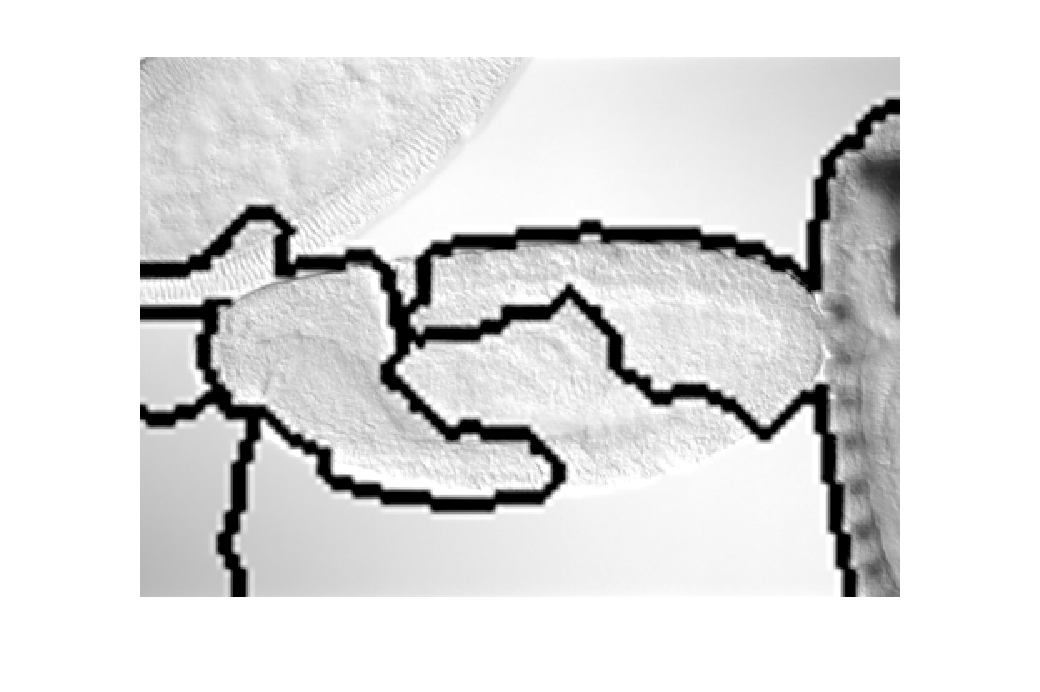
\includegraphics[scale=0.5]{hPT6_MRF1.pdf}
}
\subfigure{
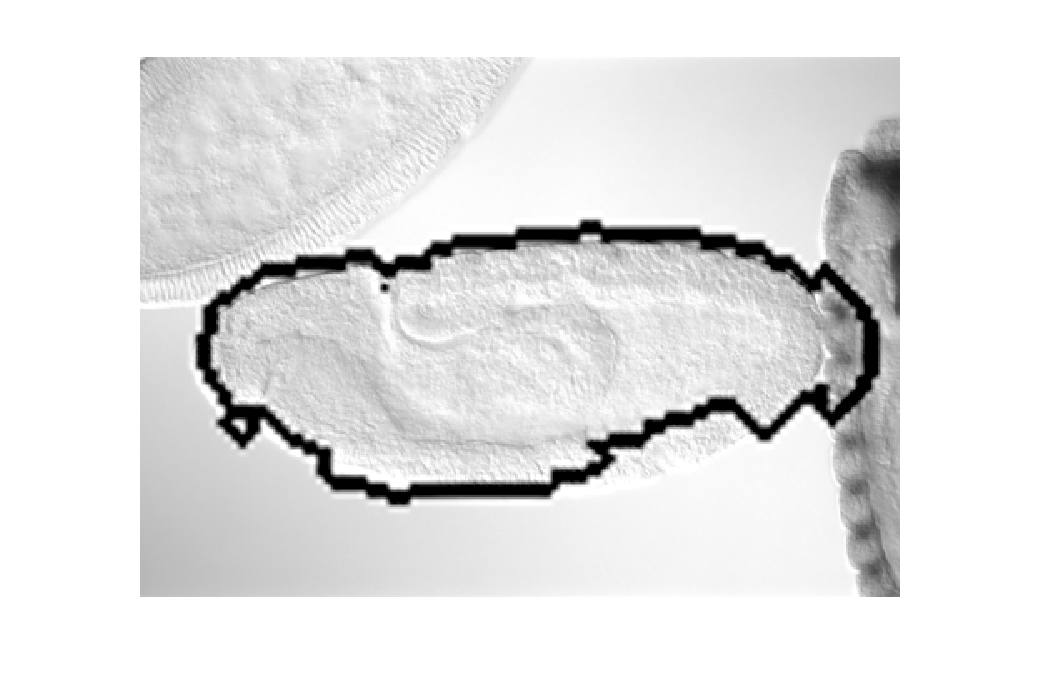
\includegraphics[scale=0.5]{hPT6_CV1.pdf}
}
\end{figure}

Result of the algorithm on test data:
1,4,5,7,8,9,

For most of the 10 test pictures, the algorithm is found to converge after less than 4 iterations. For each picture that amounts to at most 60 seconds on a ThinkPad, including running the super pixel algorithm, which is the computationally most expensive and takes 35 seconds on its 


\section{Summary and Outlook}
If we have a big enough training data set for the shape priors, in general the parameters $\mu, \sigma, \theta$ can be trained beforehand.

The next step would be to test it on the actual data set for the segmentation of the gut. 

Multilabel extension

\section{Acknowledgements}
I want to particularly thank Siqi Wu for great help in introducing me to the problem and help with the implementation process. Also I want to thank Antony Joseph, Zac Zhang and Erwin Frise for giving insights on results and problems which occurred using previous segmentation algorithms.

\FloatBarrier
\vskip 0.2in
\nocite{*}
\bibliographystyle{plain}
\bibliography{lit}

\begin{appendices}

\end{appendices}
\end{document}
